% Auto-generated by figures/src/make_captions.py (numbers from figures/src/data). Usage:
% \begin{figure*}[t]\centering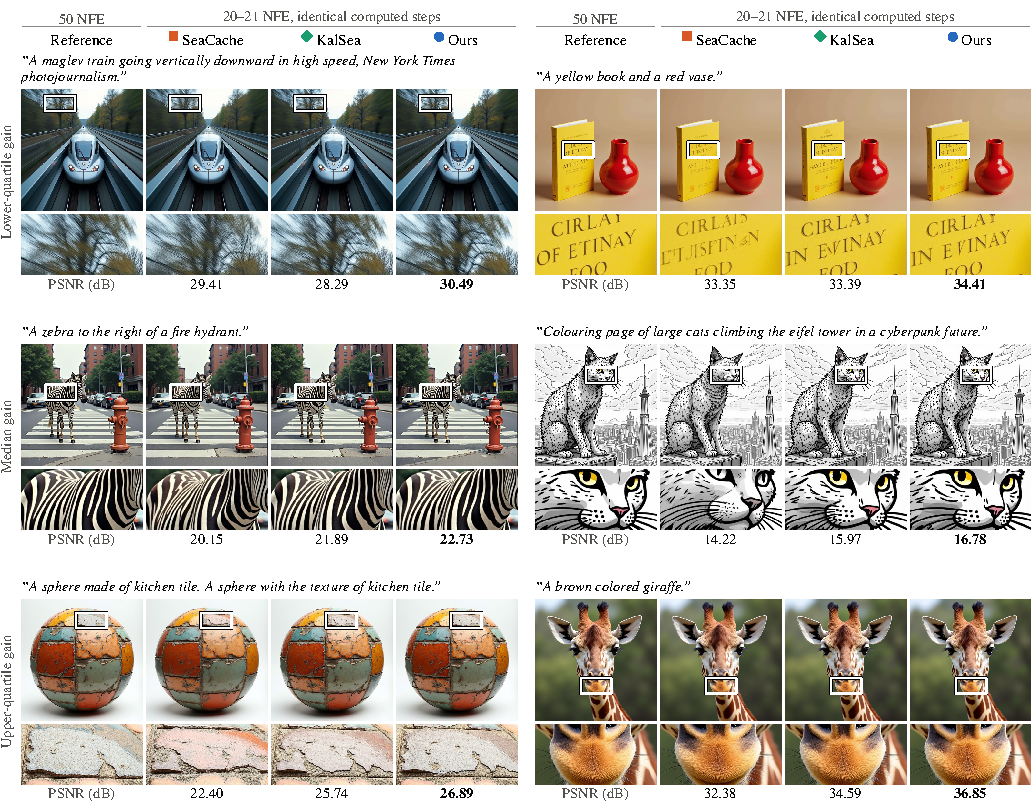
\includegraphics[width=\textwidth]{figures/fig_qualitative_supp_nfe21.pdf}% Auto-generated by figures/src/make_captions.py (numbers from figures/src/data). Usage:
% \begin{figure*}[t]\centering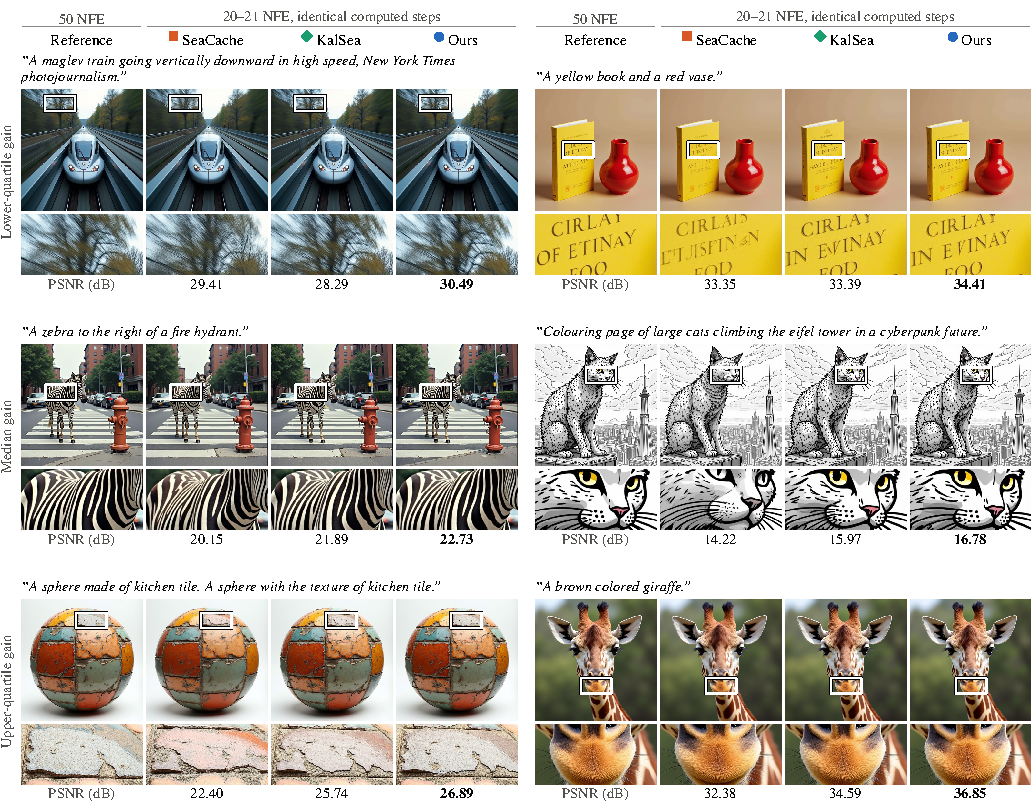
\includegraphics[width=\textwidth]{figures/fig_qualitative_supp_nfe21.pdf}% Auto-generated by figures/src/make_captions.py (numbers from figures/src/data). Usage:
% \begin{figure*}[t]\centering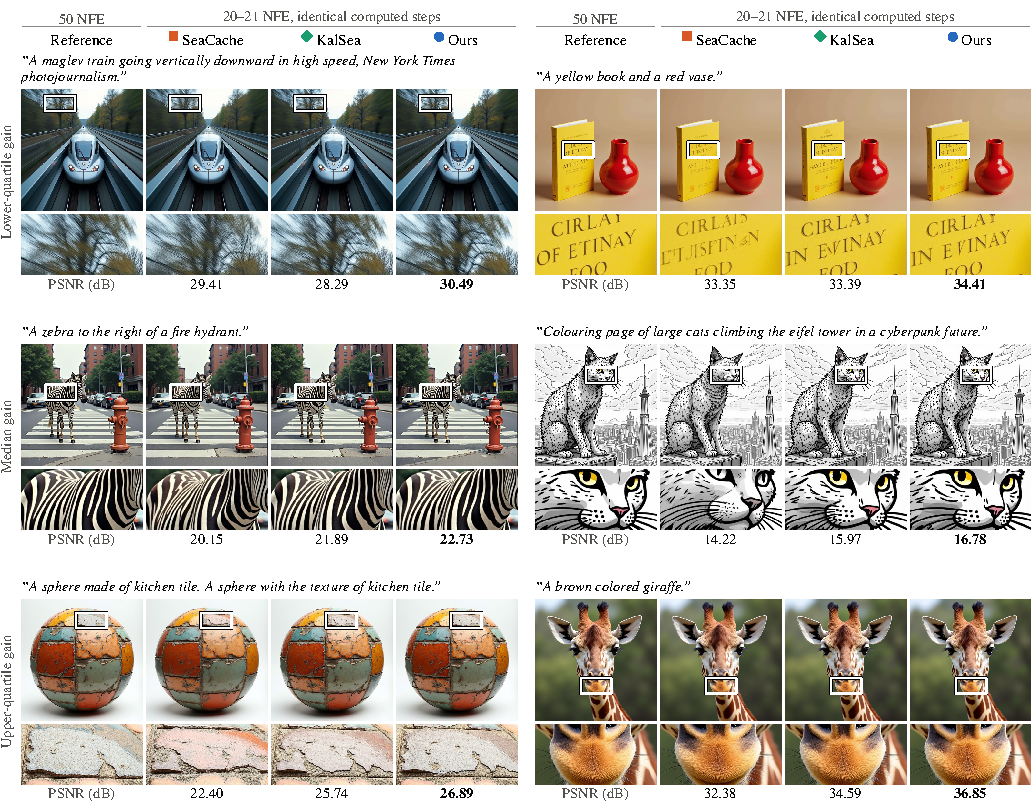
\includegraphics[width=\textwidth]{figures/fig_qualitative_supp_nfe21.pdf}% Auto-generated by figures/src/make_captions.py (numbers from figures/src/data). Usage:
% \begin{figure*}[t]\centering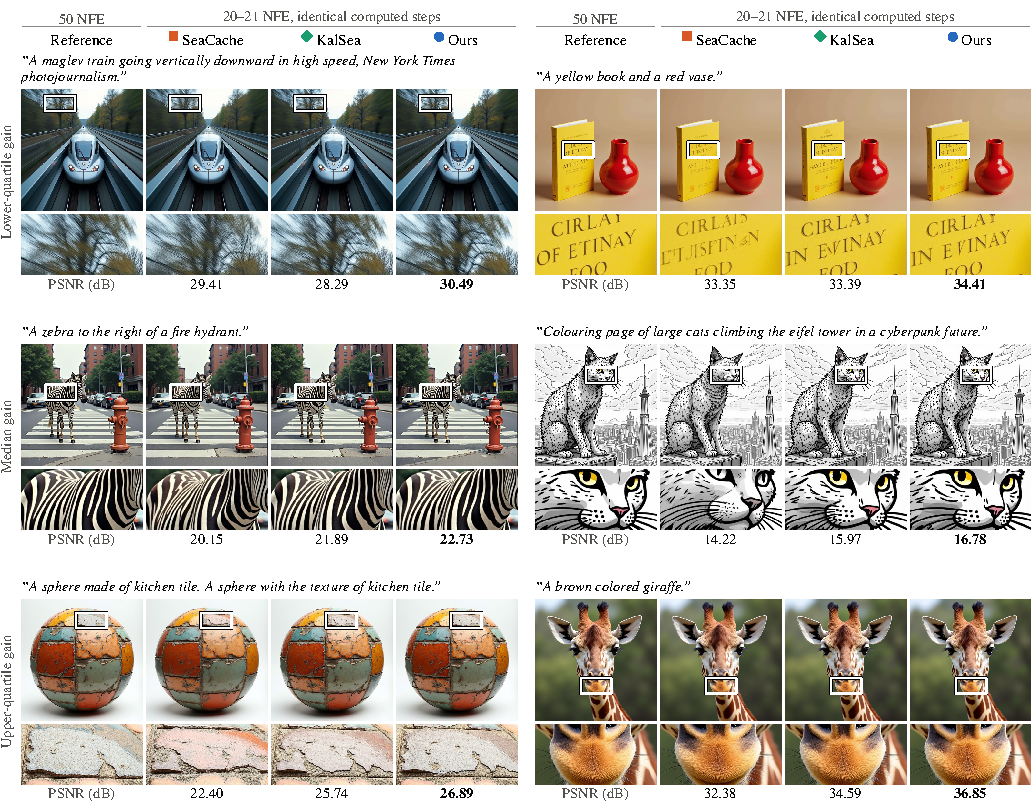
\includegraphics[width=\textwidth]{figures/fig_qualitative_supp_nfe21.pdf}\input{figures/fig_qualitative_supp_nfe21_caption}\end{figure*}
\caption{\textbf{Qualitative comparison at 20--21 \nfe (mean 20.8)} (\flux, DrawBench, $\delta = 0.3$, $2.4\times$ fewer transformer evaluations than the 50-step reference). The prompts are selected by a fixed rule, not by hand: among the 188 of 200 prompts on which \seacache, \kalsea and \ours computed the identical set of steps, we compute the per-prompt PSNR gain of \ours over \seacache and show the two prompts whose gain is closest to the lower quartile (+1.07\,dB; top row), the two closest to the median (+2.57\,dB; middle row) and the two closest to the upper quartile (+4.50\,dB; bottom row). Below each image, a fixed $256\times128$-pixel crop (of $1024\times1024$) is magnified; it is placed where the three accelerated samples differ most from one another (largest mean pairwise absolute difference), without looking at the reference. Numbers: PSNR (dB) with respect to the reference, best in bold.}
\label{fig:qualitative-supp-nfe21}
\end{figure*}
\caption{\textbf{Qualitative comparison at 20--21 \nfe (mean 20.8)} (\flux, DrawBench, $\delta = 0.3$, $2.4\times$ fewer transformer evaluations than the 50-step reference). The prompts are selected by a fixed rule, not by hand: among the 188 of 200 prompts on which \seacache, \kalsea and \ours computed the identical set of steps, we compute the per-prompt PSNR gain of \ours over \seacache and show the two prompts whose gain is closest to the lower quartile (+1.07\,dB; top row), the two closest to the median (+2.57\,dB; middle row) and the two closest to the upper quartile (+4.50\,dB; bottom row). Below each image, a fixed $256\times128$-pixel crop (of $1024\times1024$) is magnified; it is placed where the three accelerated samples differ most from one another (largest mean pairwise absolute difference), without looking at the reference. Numbers: PSNR (dB) with respect to the reference, best in bold.}
\label{fig:qualitative-supp-nfe21}
\end{figure*}
\caption{\textbf{Qualitative comparison at 20--21 \nfe (mean 20.8)} (\flux, DrawBench, $\delta = 0.3$, $2.4\times$ fewer transformer evaluations than the 50-step reference). The prompts are selected by a fixed rule, not by hand: among the 188 of 200 prompts on which \seacache, \kalsea and \ours computed the identical set of steps, we compute the per-prompt PSNR gain of \ours over \seacache and show the two prompts whose gain is closest to the lower quartile (+1.07\,dB; top row), the two closest to the median (+2.57\,dB; middle row) and the two closest to the upper quartile (+4.50\,dB; bottom row). Below each image, a fixed $256\times128$-pixel crop (of $1024\times1024$) is magnified; it is placed where the three accelerated samples differ most from one another (largest mean pairwise absolute difference), without looking at the reference. Numbers: PSNR (dB) with respect to the reference, best in bold.}
\label{fig:qualitative-supp-nfe21}
\end{figure*}
\caption{\textbf{Qualitative comparison at 20--21 \nfe (mean 20.8)} (\flux, DrawBench, $\delta = 0.3$, $2.4\times$ fewer transformer evaluations than the 50-step reference). The prompts are selected by a fixed rule, not by hand: among the 188 of 200 prompts on which \seacache, \kalsea and \ours computed the identical set of steps, we compute the per-prompt PSNR gain of \ours over \seacache and show the two prompts whose gain is closest to the lower quartile (+1.07\,dB; top row), the two closest to the median (+2.57\,dB; middle row) and the two closest to the upper quartile (+4.50\,dB; bottom row). Below each image, a fixed $256\times128$-pixel crop (of $1024\times1024$) is magnified; it is placed where the three accelerated samples differ most from one another (largest mean pairwise absolute difference), without looking at the reference. Numbers: PSNR (dB) with respect to the reference, best in bold.}
\label{fig:qualitative-supp-nfe21}
